%!TEX root = ../thesis.tex
\chapter{Results}
\label{ch:results}

\begin{itemize}
    \item Konsistenz aller Modelle über die 5 Folds der Kreuzvalidierung ist gut, was eine robuste Trainierbarkeit bedeutet
\end{itemize}
\section{Oriented Bounding Boxes and Axis Aligned Bounding Boxes}
\begin{itemize}
    \item Training Results by the mAP50-95 of all 5 Folds for every model 
    \item Left Side (Blue): Yolov9 (without obb) and with axis aligned Bounding Boxes
    \item Middle (Orange): Yolov9u with oriented bounding boxes
    \item Uses Ultralytics as Backend for obb support
    \item Right (Green): Yolov9u with axis aligned Bounding Boxes in the oriented Bounding Box format
    \item Result -> aab performs better
    \item \todo{Vergleichsbild eifnügen oder verweis}
    \item This is probably due to the fact that small changes in the orientation of the bounding boxes lead to a greater deviation of the mean average precision 
    \item Oriented Bounding boxes are smaller than the axis aligned bounding boxes -> higher inaccuracy of mAP50-95 (see next slide)
    \item Red box at the right picture has a small deviation from the correct (blue) label
\end{itemize}
\begin{itemize}
    \item \todo{Bild für Vergleich der BB Area einfügen (zw. obb, aab aab old)}
    \item Oriented Bounding Boxes has an area from around 600 to 900 pixels 
    \item Axis aligned Bounding boxes from around 750 to 1300 px
    \item-> higher inaccuracy of mAP50-95

    \item For the channel permutation I used the obb model

\end{itemize}

\section{Comparision at Mean Average Precision 50-95}

\begin{itemize}
    \item \todo{Bild einfügen best val dataset on val data}
    \item See the performance of the best validation model on the validation data (per fold and model)
    \item RGBIR has the best performance followed by irgb 
    \item 3. place are rgb and rirb
    \item Rgir and both ndvi models has the poorest map values
\end{itemize}

\begin{itemize}
    \item \todo{Bild einfügen; best val dataset on test data}
    \item Best Validation Models on the test data (Fold 5)
    \item Red Dots are the best validation model at the validation data on the test data
    \item (means the highest whisker from the previous slide)
    \item Difference between the quantils, rgir performs at best
    \item Then the rirb model and rgb model 
\end{itemize}

\begin{itemize}
    \item \todo{Tabelle einfügen}
    \item Difference Between best mAP Fold at the validation data
    \item From 0 to 4
    \item Smaller difference at the mAP Performance at the test data
    \item Fold 2 and 3
    \item Now looking at the confusion and difference matrices
\end{itemize}



\section{Comparision with Confusion Matrices}
\begin{itemize}
    \item \todo{beide confusionsmatricen einfügen}
    \item Normalisierte Konfusions Matrix mit 9 Klassen und der Einteilung Background (Hintergrund)
    \item Right: Confusion Matric of RGBIR Modell on Fold 2:
    \item Good Performance at Cars, Trucks, Ships, Tractors, Camping Cars, Pick Up and planes
    \item Many confusion at vehicle with background
    \item Nearly the same for RGIR at Fold 3
    \item Both modells detected nearly all Planes
    \item Difference Matrics at next slide
\end{itemize}

\begin{itemize}
    \item \todo{Differenzmatrix RGBIR vs RGIR einfügen}
    \item At all Difference Matrices is red for the better performance of the RGBIR Model and blue for the other modell
    \item RGBIR detected Trucks, Ships and Tractor more accurate than the RGIR Model
    \item RGBIR seems more robust for common ground vehicles
    \item Both modells detect all planes (in short every modell detect all planes)
    \item Both modells misclassifier background as any class (RGBIR is better at vehicle and Camping Car) 
\end{itemize}

\begin{itemize}
    \item \todo{Differenzmatrix RGBIR vs RGB einfügen}
    \item RGBIR is better for detecting Ships (12\%) and Vehicles (15\%), slightliy degrades performance of car detection
    \item Vehicle is much better than in RGB Model (15\%)
    \item IR input helps for common vehicle recognition (vehicle includes Excavators, construction equipment, etc.)
    \item RGB is better in identifying ship and vehicle as background
\end{itemize}


\begin{itemize}
    \item \todo{Differenzmatrix RGBIR vs IRGB einfügen}
    \item RGBIR recognize Ships 21 \% better than the irgb model
    \item Particulary stronger for camping car and van classification (6\%)
    \item IRGB has more  background-ship and background-vehicle confusion
\end{itemize}

\begin{itemize}
    \item \todo{Differenzmatrix RGBIR vs RIRB einfügen}
    \item RGBIR detects Ships and vans better than RIRB Model
    \item RIRB misclassified van and ship as background more often than RGBIR

\end{itemize}


\begin{itemize}
    \item \todo{Differenzmatrix RGBIR vs GBNDBVI und RGBNDVI einfügen}
    \item RGBIR have a better performance in Ship, Tractor and Vehicle
    \item Both ndvi modells show  a tendency for confusing background with other classes
\end{itemize}

\section{Ablation Studies}
% \begin{figure}[h] 
%     \centering
%     % Erste Subfigur
%     \begin{subfigure}[b]{0.85\textwidth} % [b] für bottom alignment, 0.48\textwidth damit noch Platz ist
%         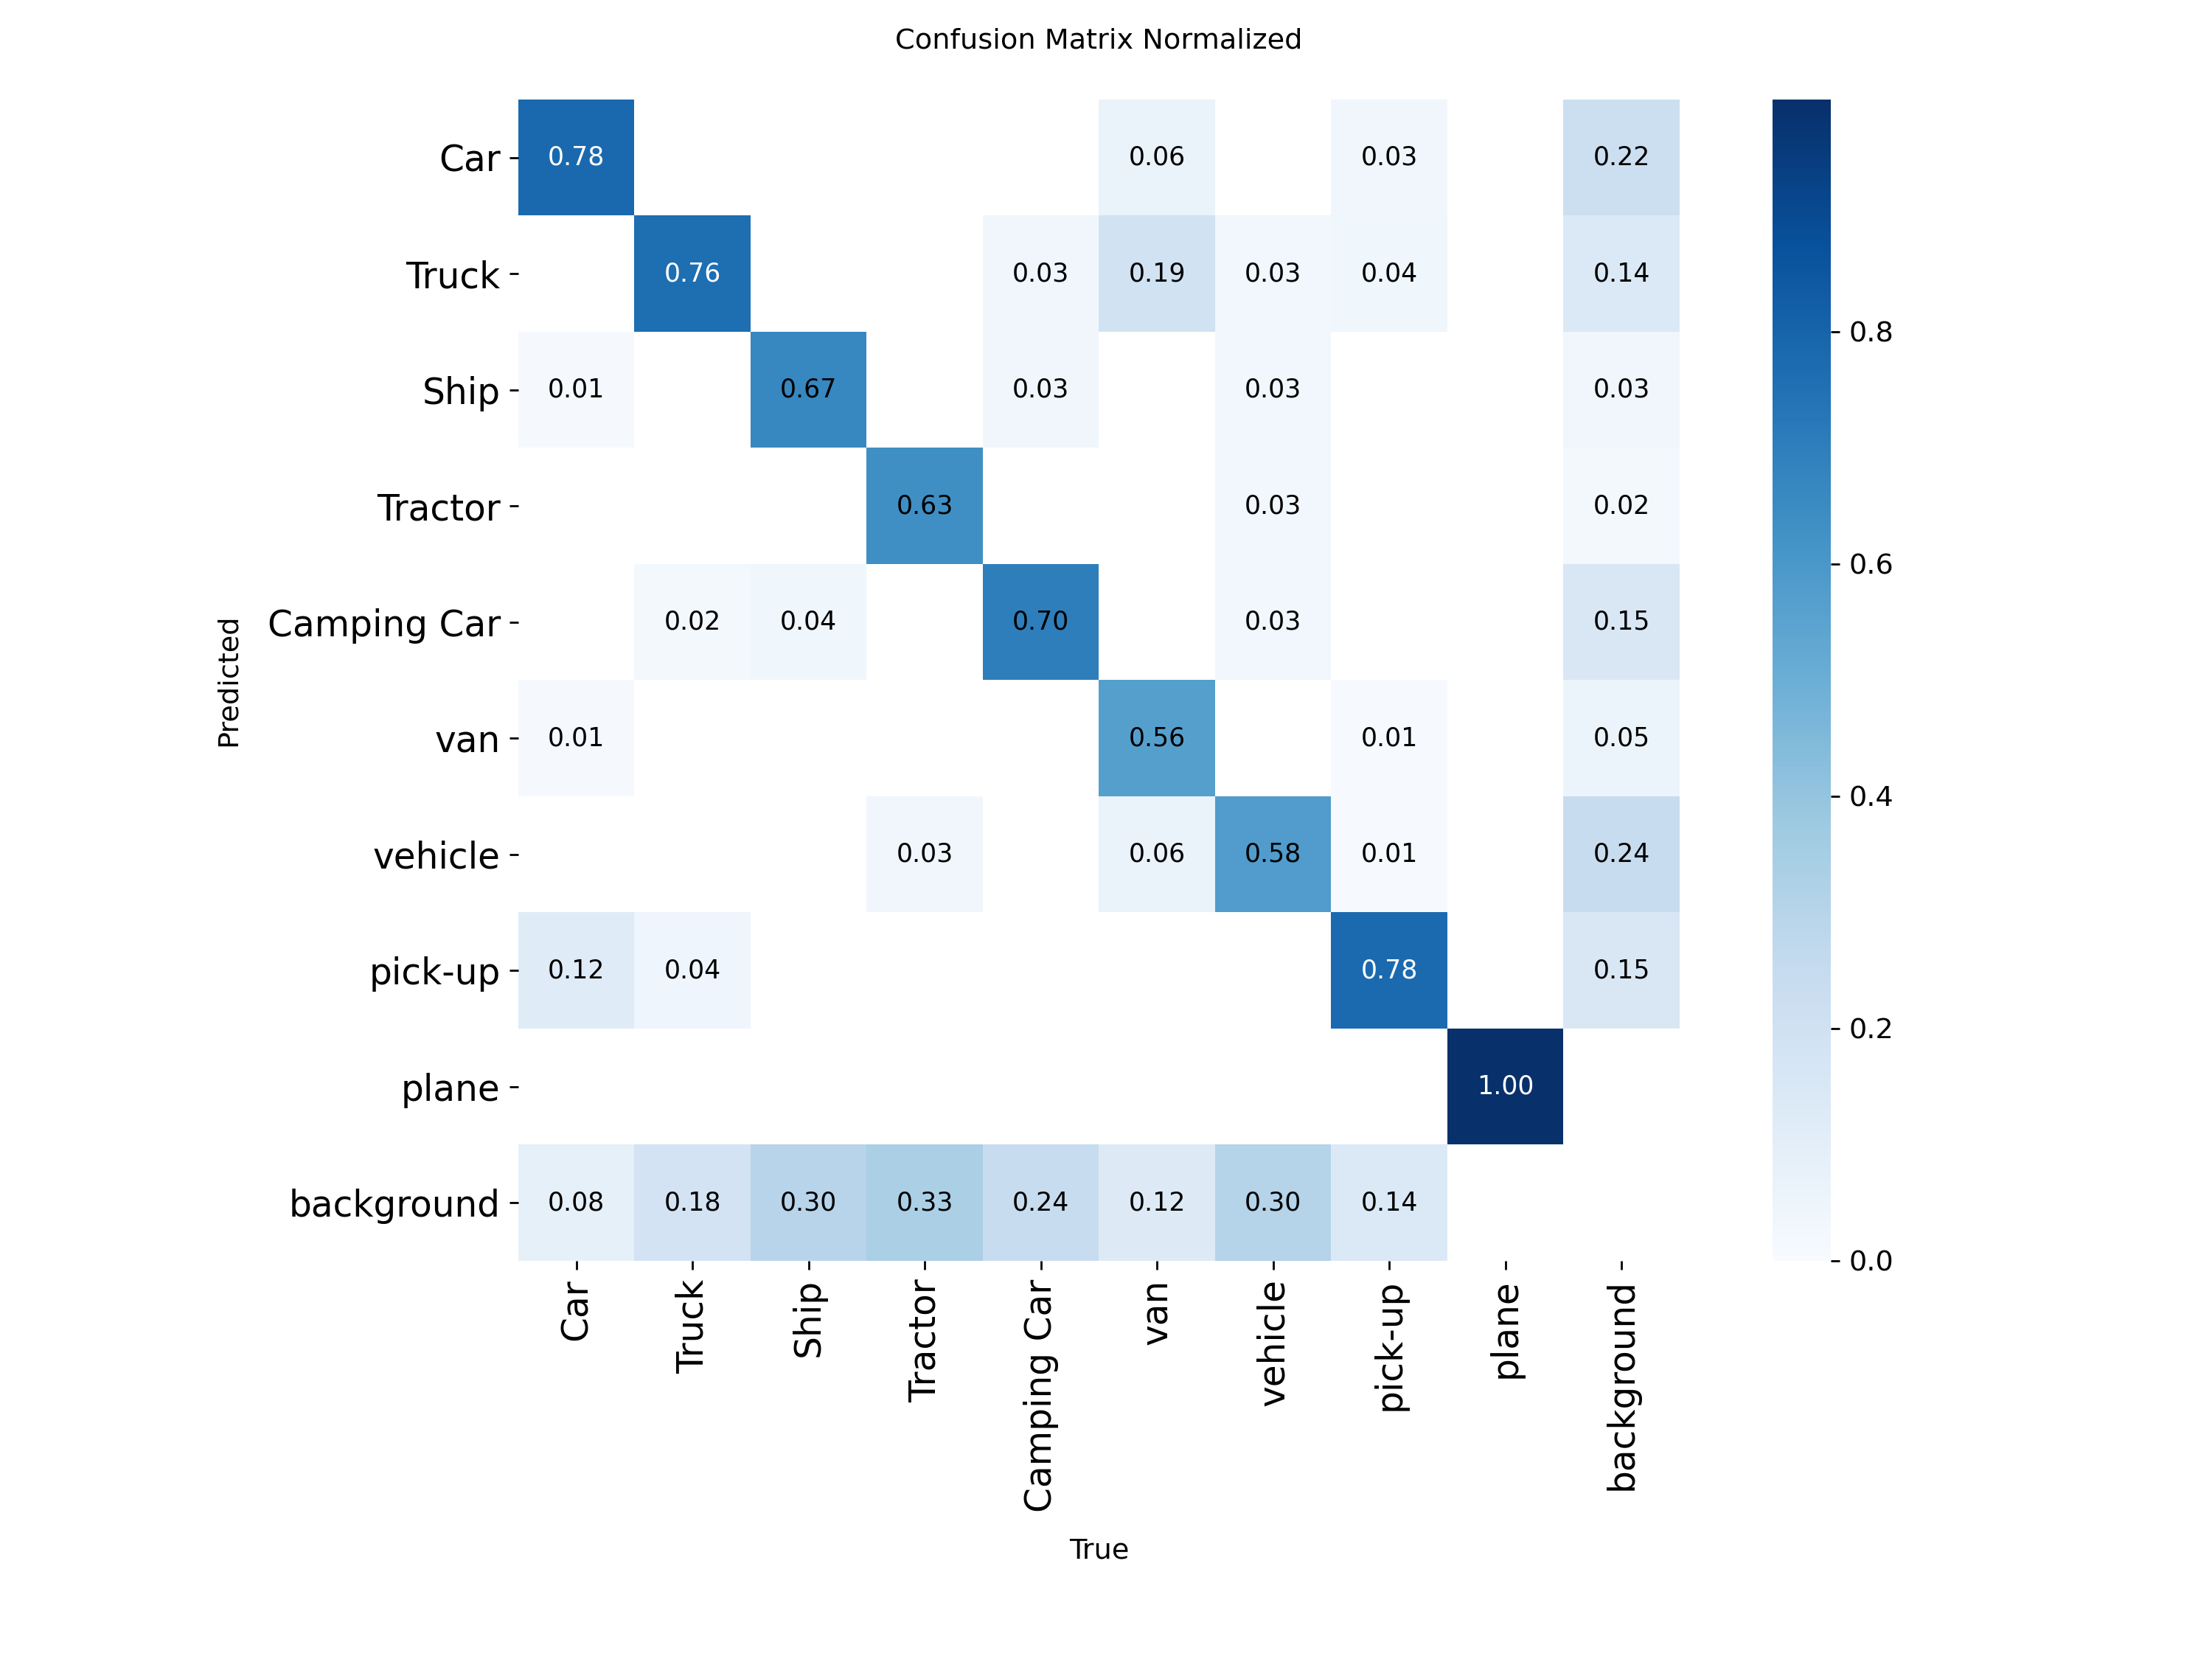
\includegraphics[width=\textwidth]{images/confusion_matrices/rgbir_F4_confusion_matrix_normalized.png} % Bildpfad zum ersten Bild
%         \caption{r-g-b-ir} % Unterschrift für das erste Bild
%         \label{fig:cm_rgbir} % Label für Referenzierung von Bild 1
%     \end{subfigure}
%     \hfill % Fügt horizontalen Platz zwischen den Subfiguren ein
%     % Zweite Subfigur
%     \begin{subfigure}[b]{0.85\textwidth} % 0.48\textwidth für das zweite Bild
%         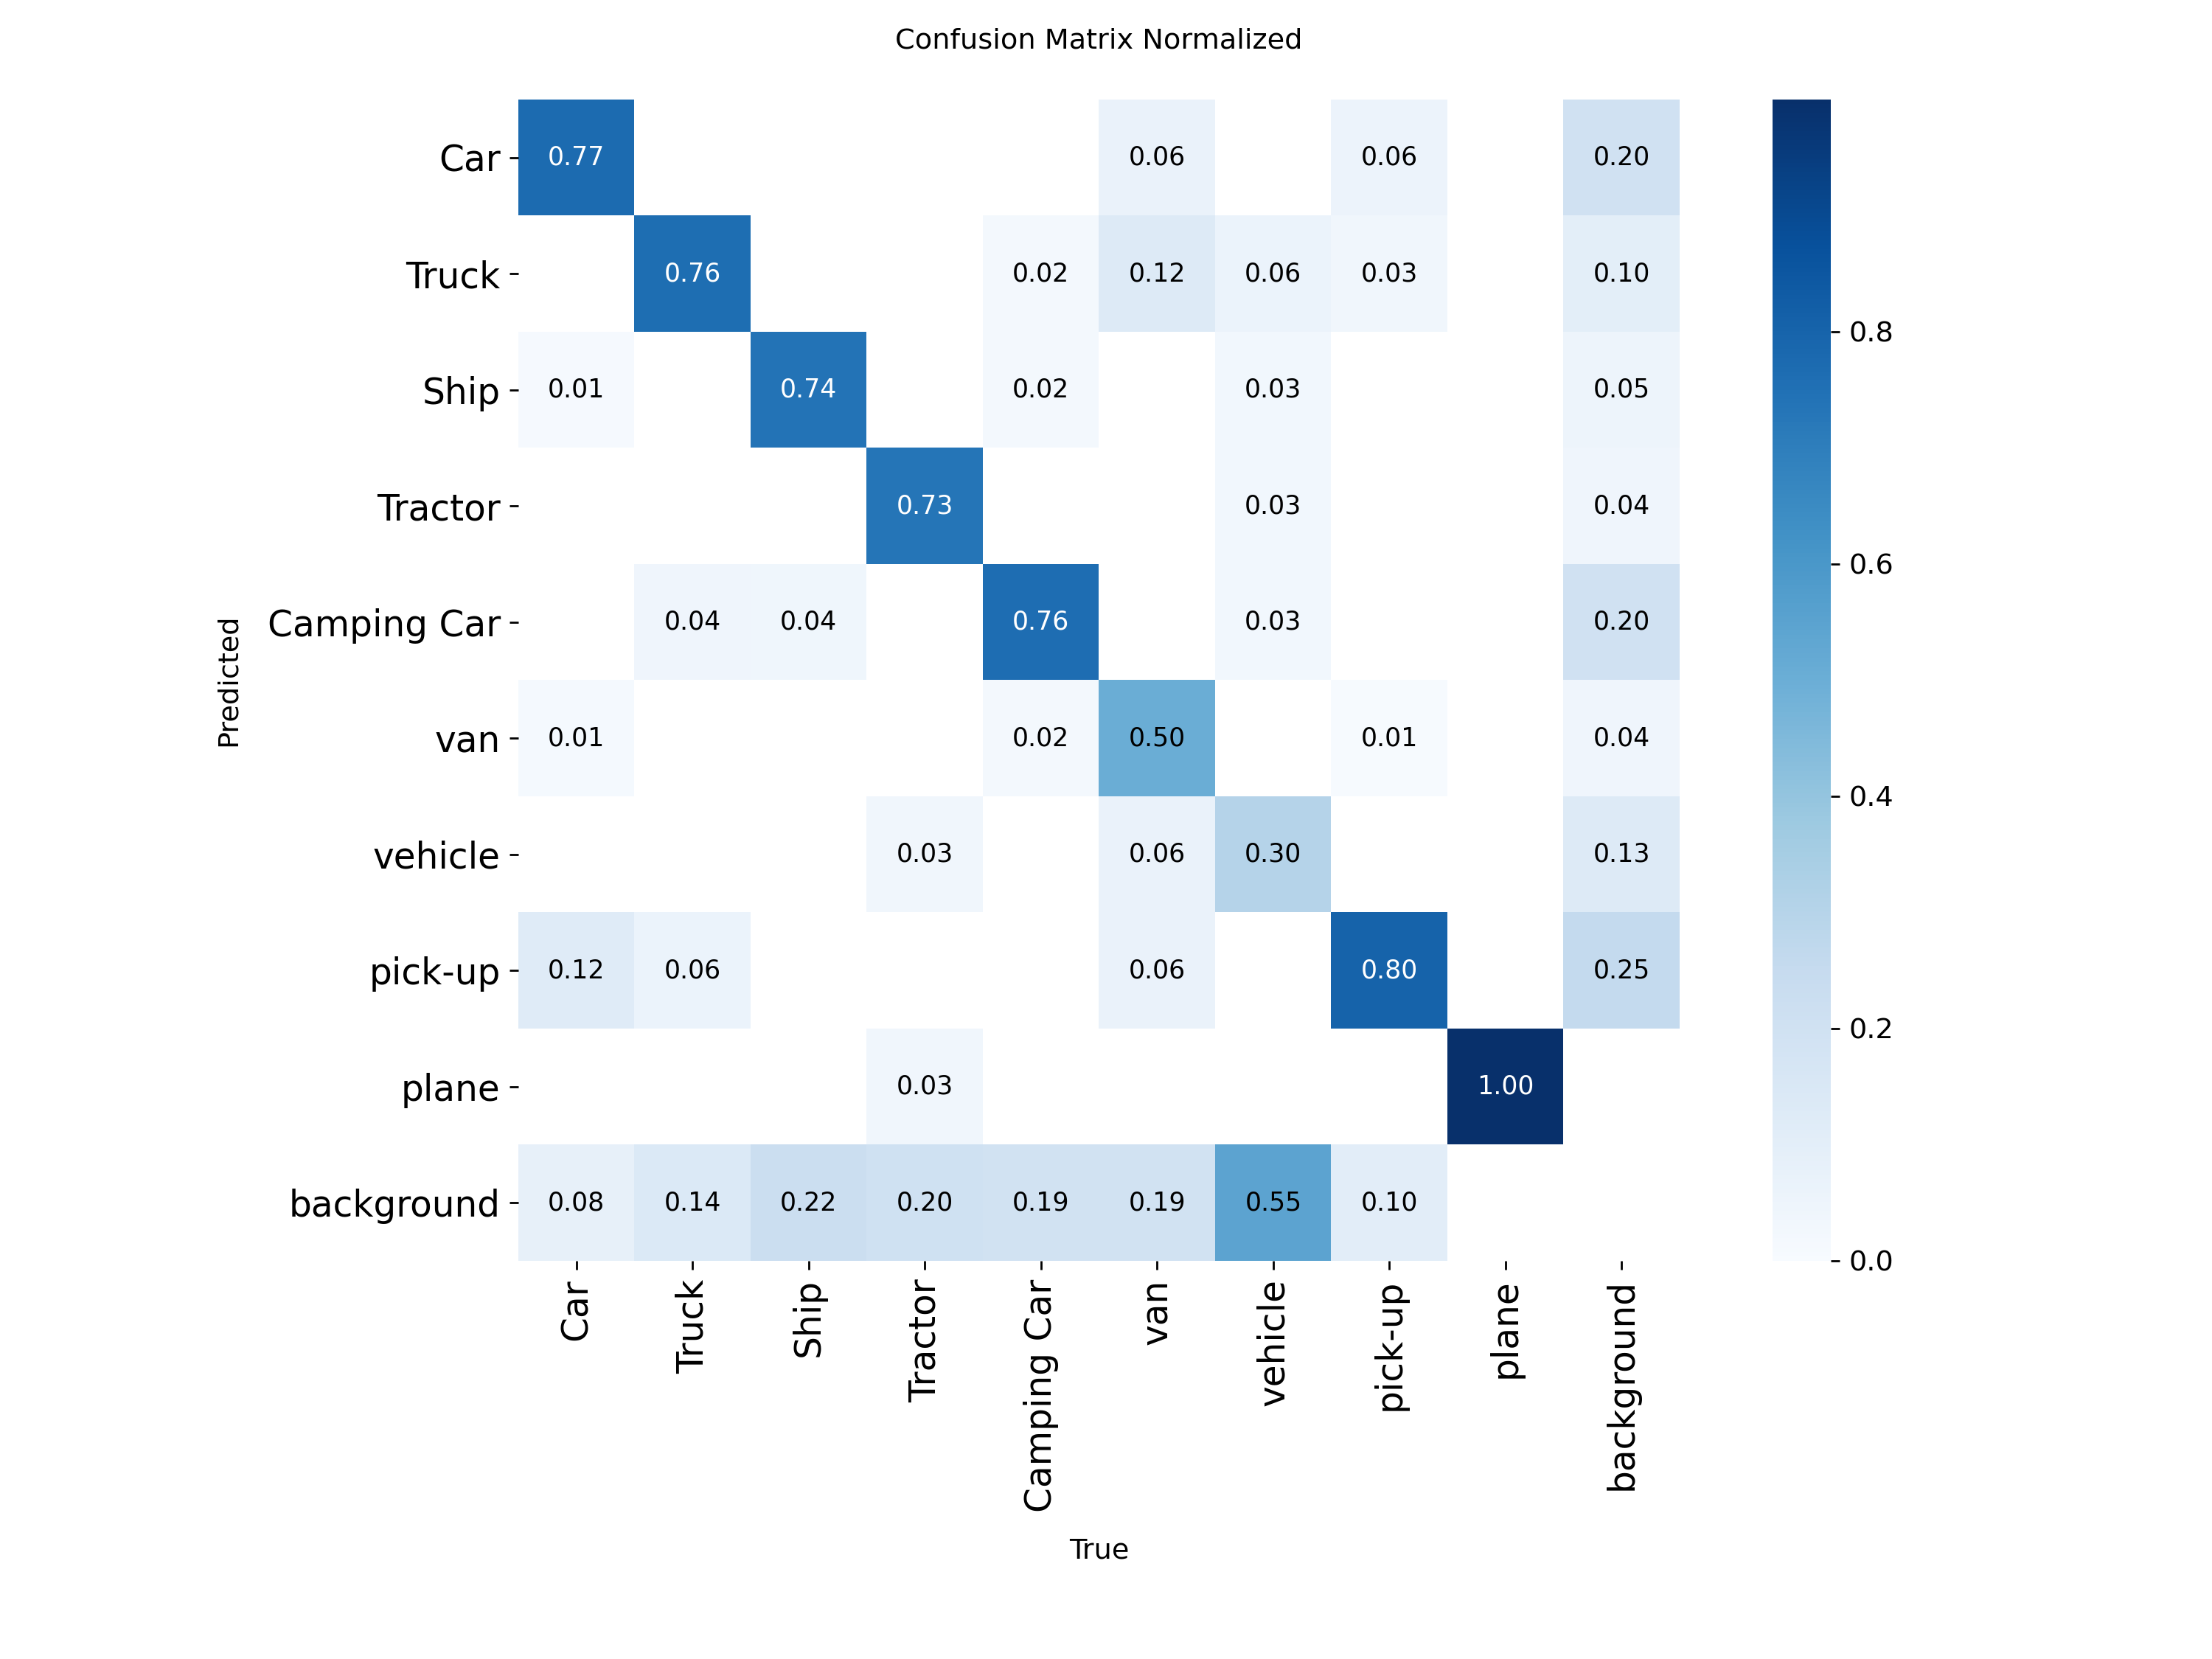
\includegraphics[width=\textwidth]{images/confusion_matrices/irgb_F4_confusion_matrix_normalized.png} % Bildpfad zum zweiten Bild
%         \caption{ir-g-b} % Unterschrift für das zweite Bild
%         \label{fig:cm_irgb} % Label für Referenzierung von Bild 2
%     \end{subfigure}
%     \caption{Comparison of Confusion Matrices between r-g-b-ir und ir-g-b for Fold 4} % Gemeinsame Unterschrift für beide Bilder
%     \label{fig:combined_maps} % Label für die gesamte Figure-Umgebung
% \end{figure}

% \begin{figure}[h] 
%     \centering
%     % Erste Subfigur
%     \begin{subfigure}[b]{0.85\textwidth} % [b] für bottom alignment, 0.48\textwidth damit noch Platz ist
%         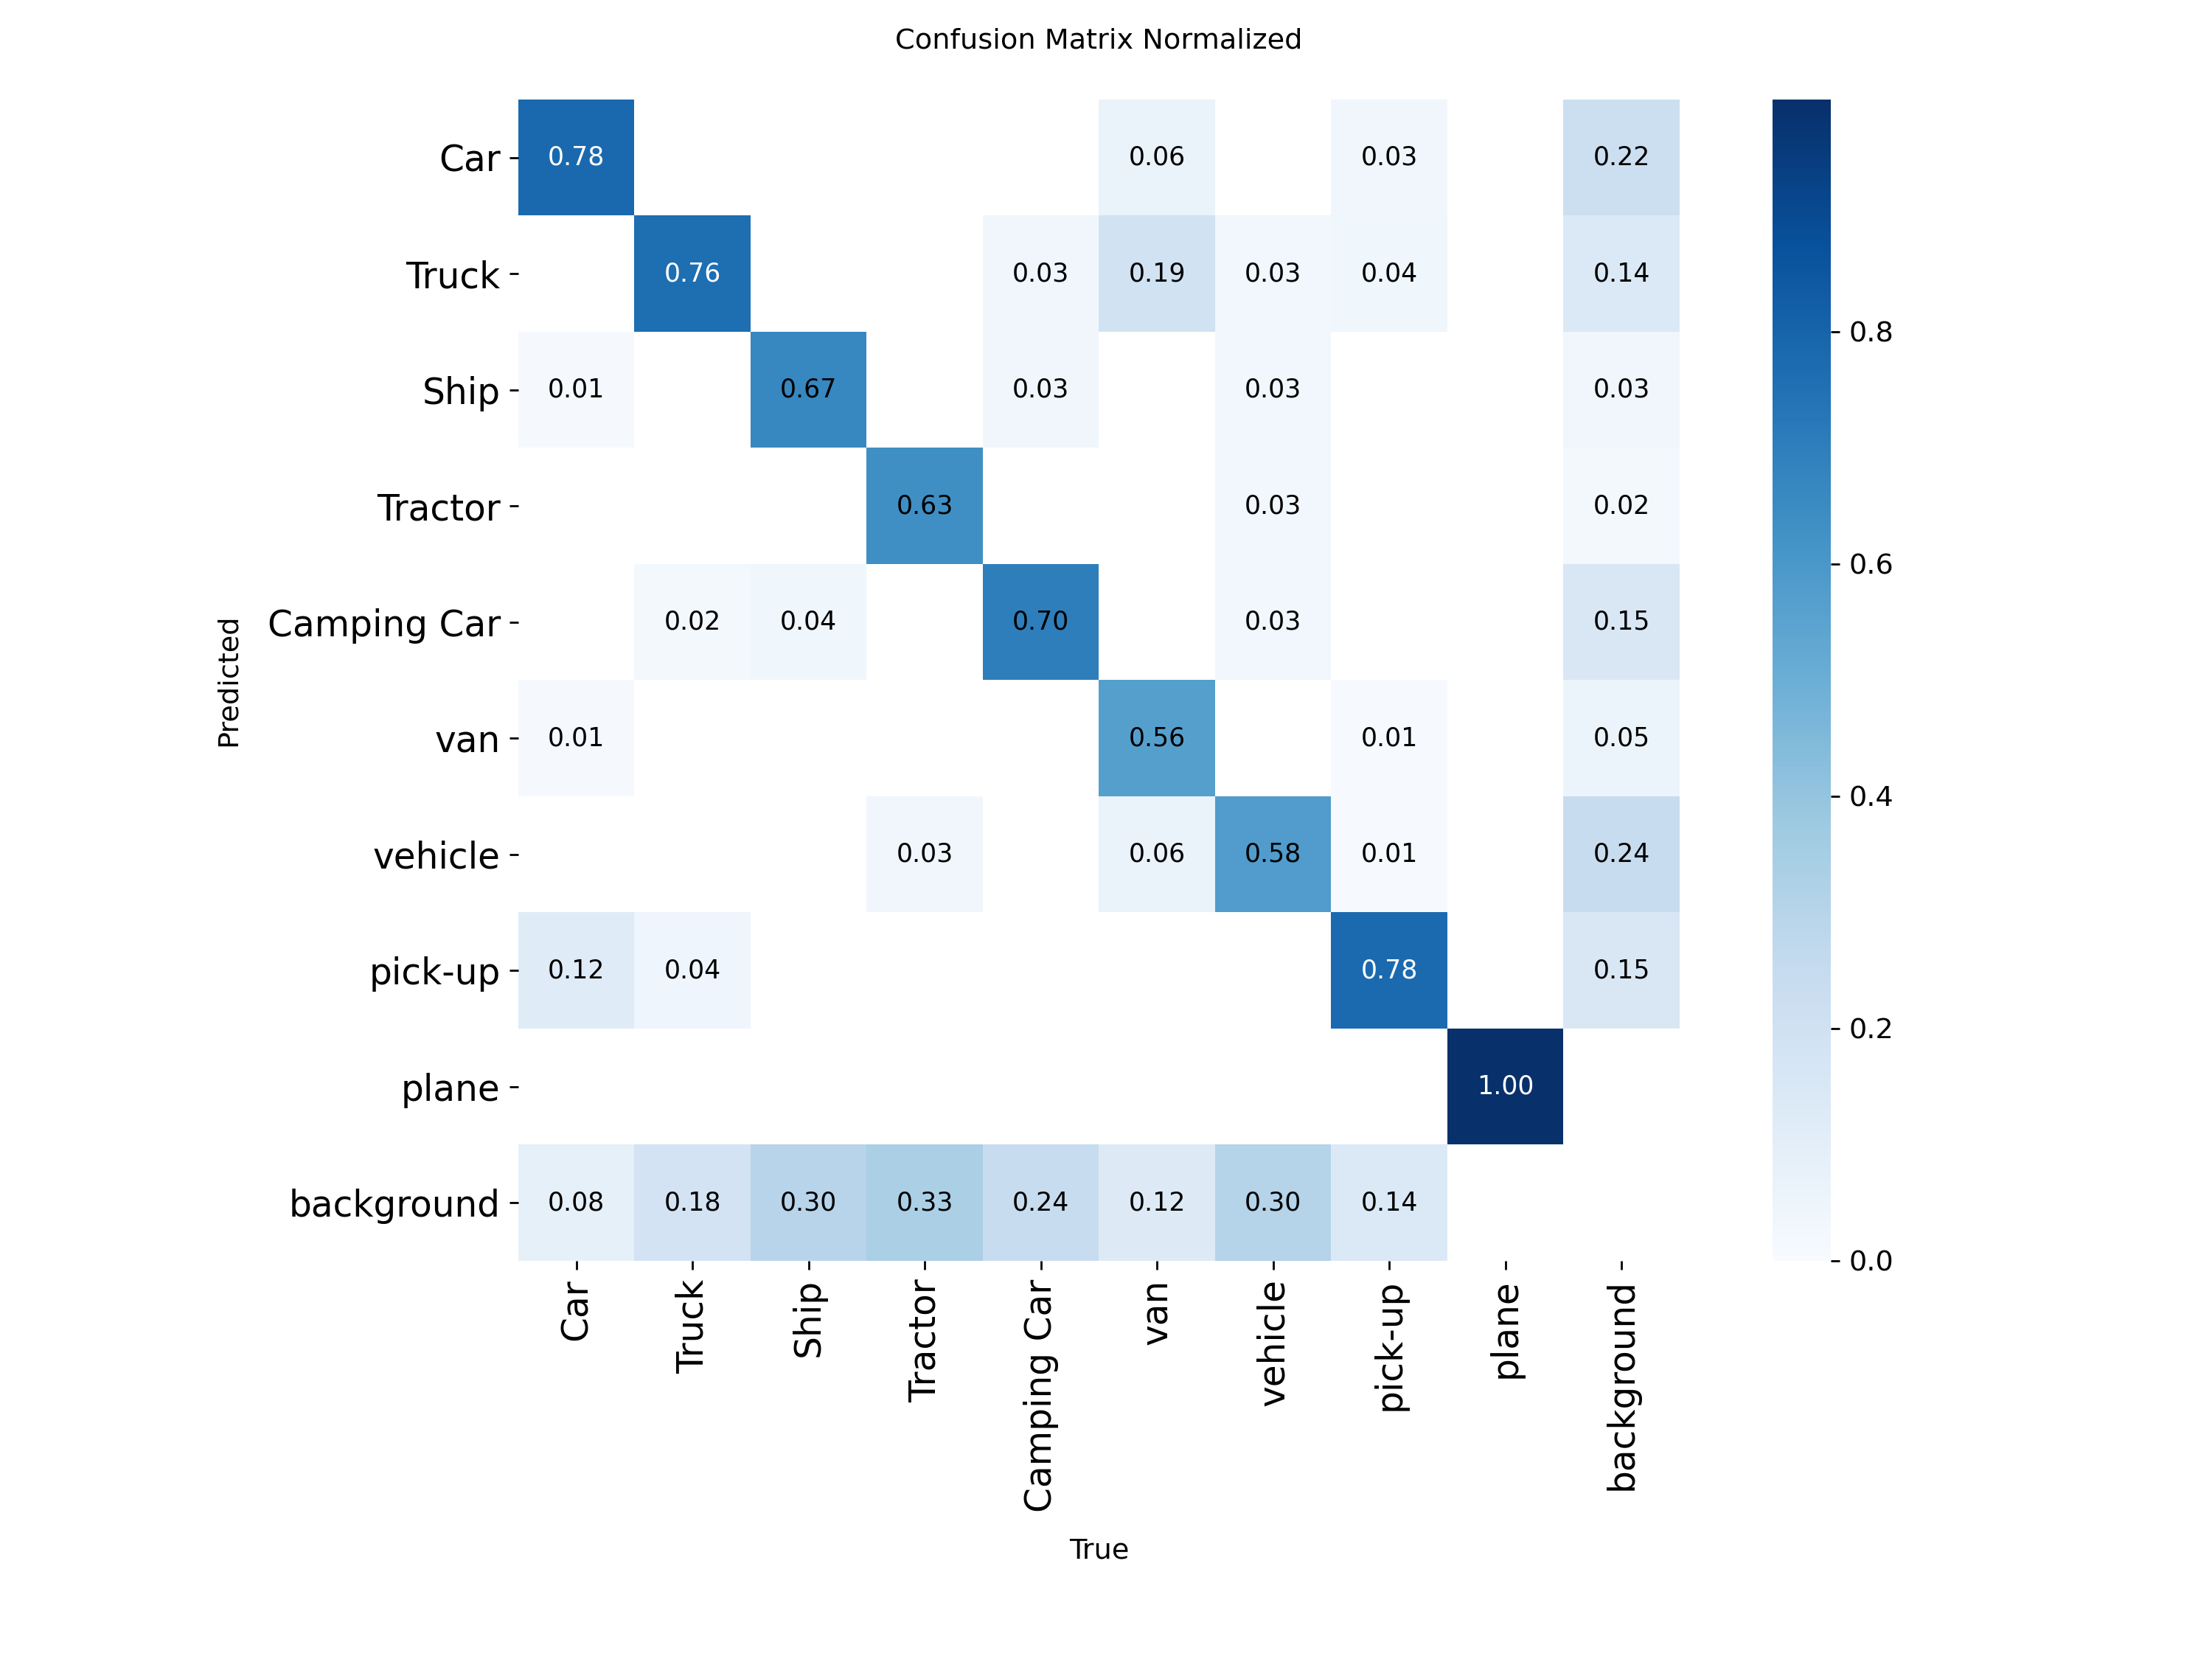
\includegraphics[width=\textwidth]{images/confusion_matrices/rgbir_F4_confusion_matrix_normalized.png} % Bildpfad zum ersten Bild
%         \caption{r-g-b-ir} % Unterschrift für das erste Bild
%         \label{fig:cm_trgbir} % Label für Referenzierung von Bild 1
%     \end{subfigure}
%     \hfill % Fügt horizontalen Platz zwischen den Subfiguren ein
%     % Zweite Subfigur
%     \begin{subfigure}[b]{0.85\textwidth} % 0.48\textwidth für das zweite Bild
%         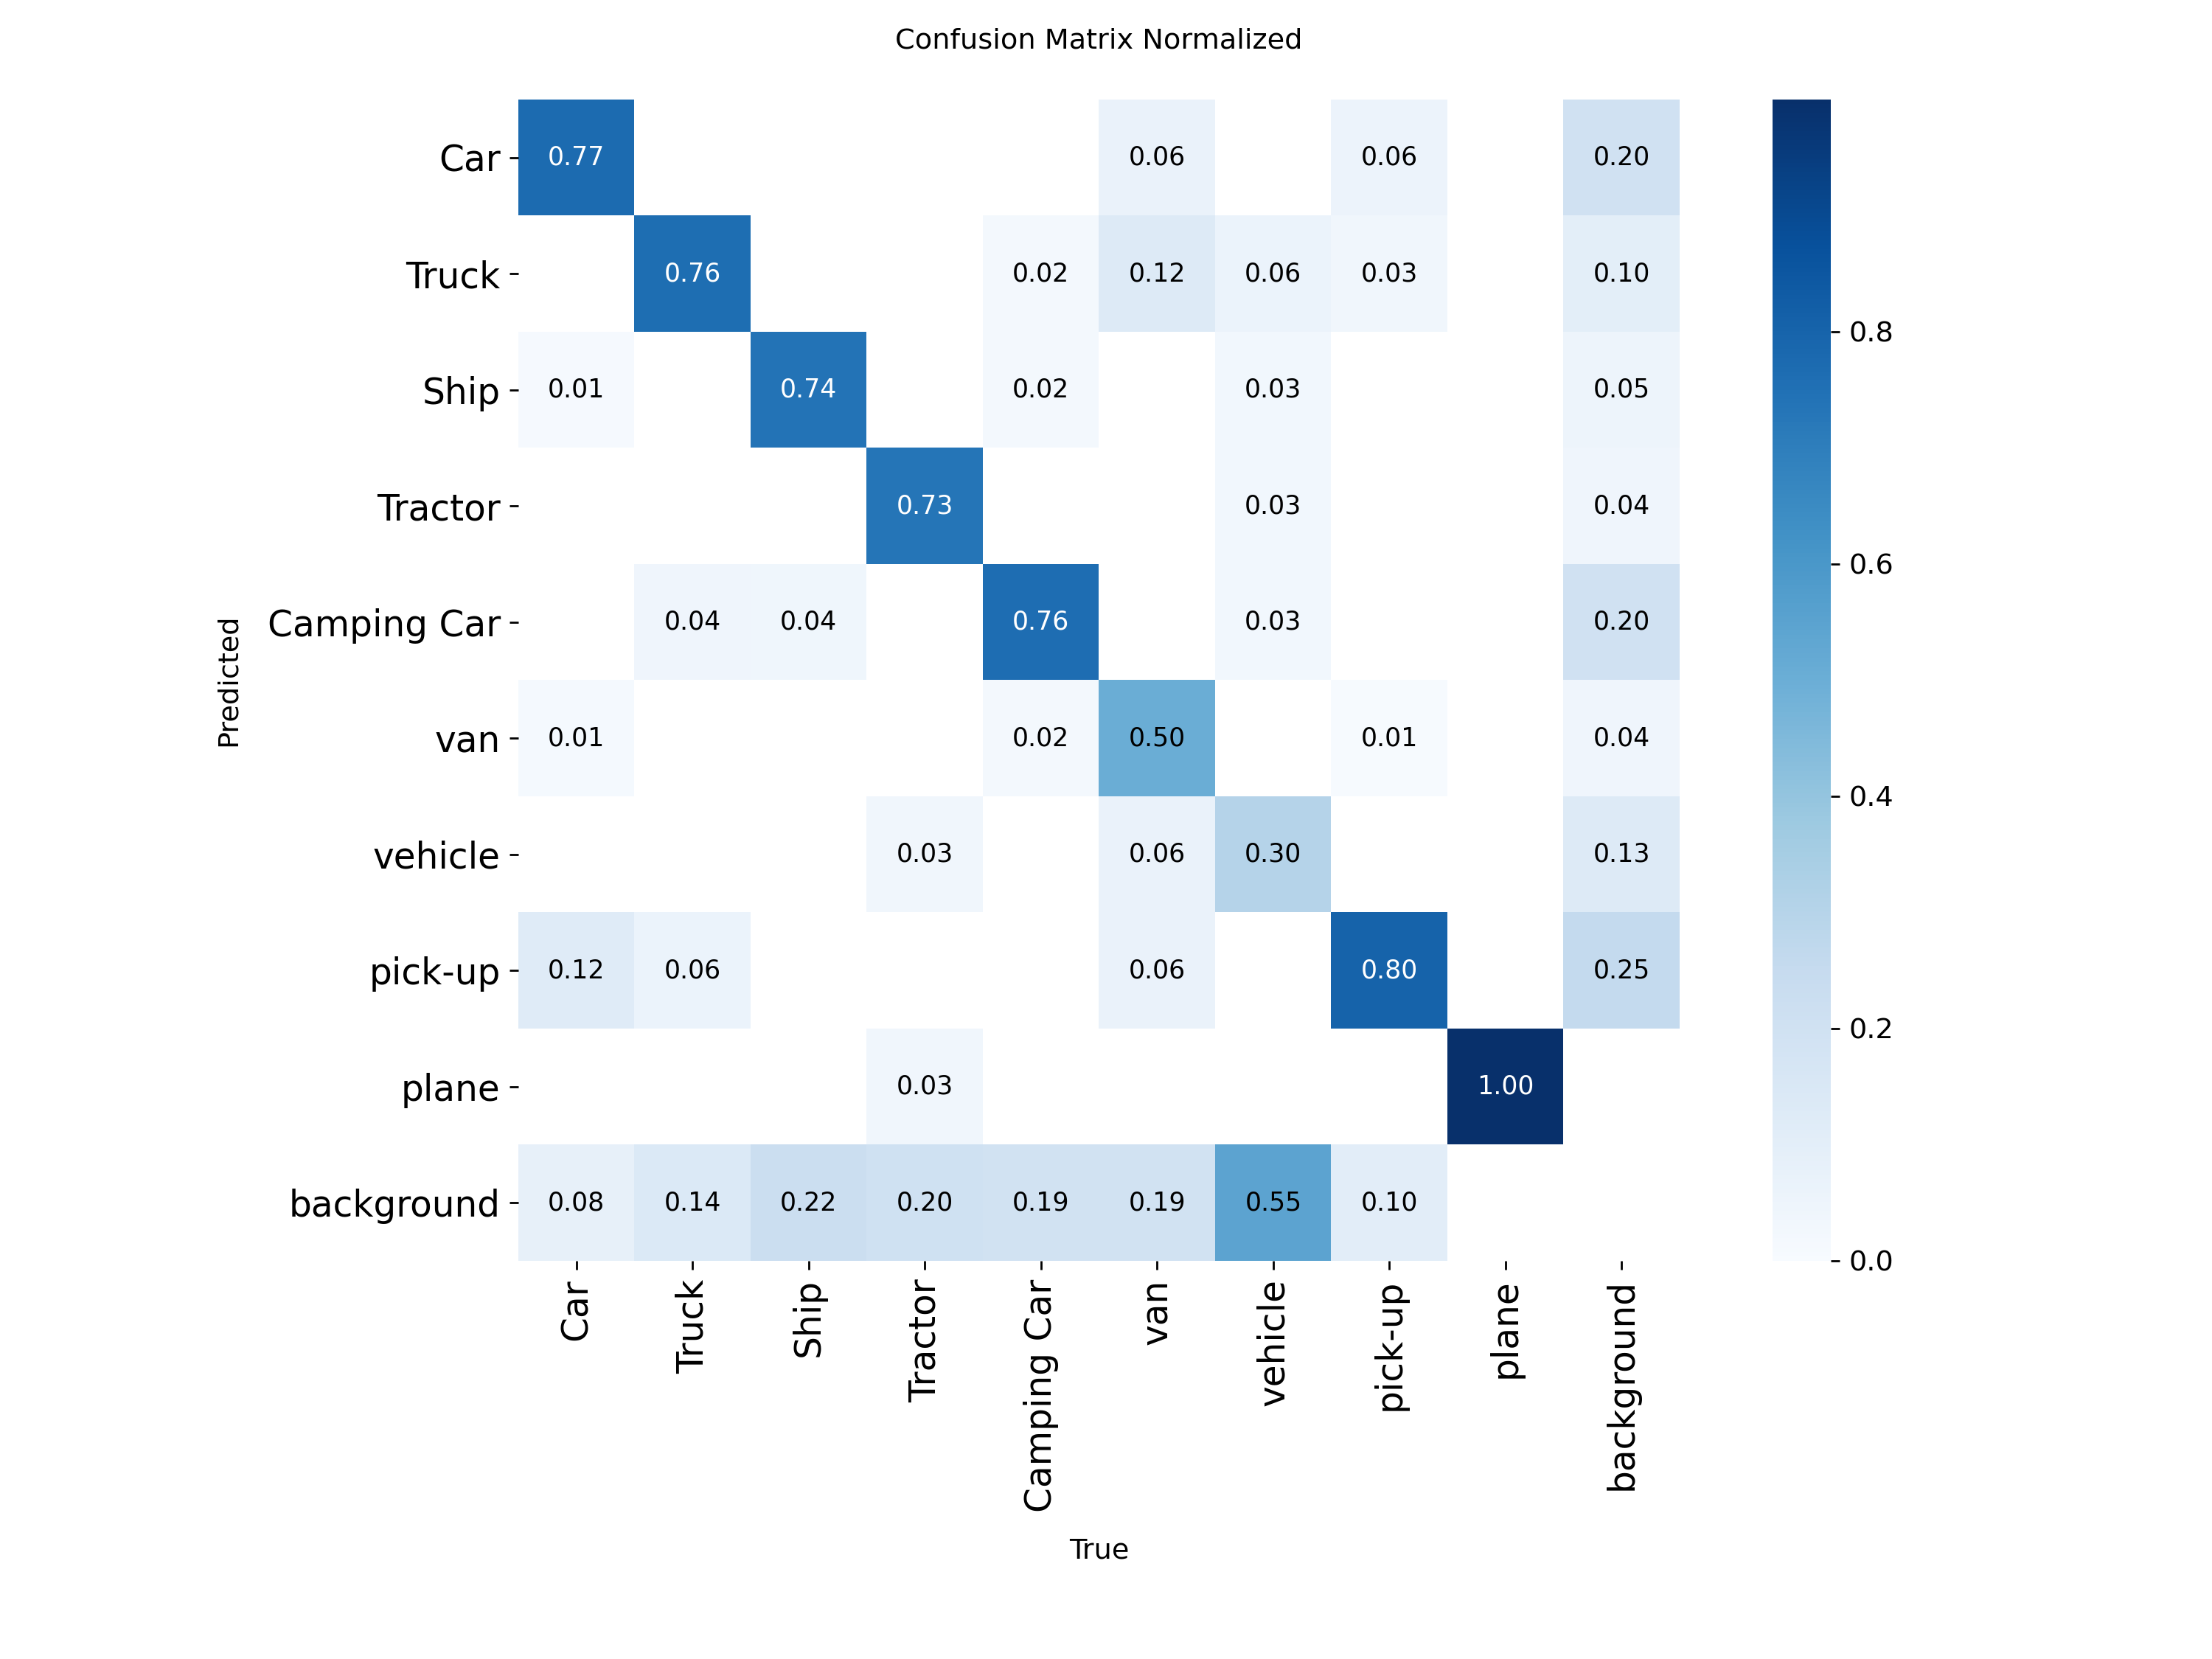
\includegraphics[width=\textwidth]{images/confusion_matrices/irgb_F4_confusion_matrix_normalized.png} % Bildpfad zum zweiten Bild
%         \caption{ir-g-b} % Unterschrift für das zweite Bild
%         \label{fig:cm_irgb} % Label für Referenzierung von Bild 2
%     \end{subfigure}
%     \caption{Comparison of Confusion Matrices between r-g-b-ir und ir-g-b for Fold 4} % Gemeinsame Unterschrift für beide Bilder
%     \label{fig:combined_maps} % Label für die gesamte Figure-Umgebung
% \end{figure}